\documentclass[a4paper,12pt]{article}
\usepackage[utf8]{inputenc}
\usepackage[T1]{fontenc}
\usepackage[spanish]{babel}
\usepackage{csquotes}
\usepackage{anysize}
\usepackage{graphicx}
\marginsize{25mm}{25mm}{25mm}{25mm}

\title{Irrational choice and the value of information}
\author{Marco Vasconcelos, Tiago Monteiro, Alex Kacelnik}
\date{2015}

\begin{document}

{\scshape\bfseries \maketitle}

Los casos de conducta aparentemente irracional plagan la literatura y parecen plantear dudas sobre el uso de la teoría de optimalidad. La irracionalidad se interpreta como sesgos cognitivos o heurísticos ad-hoc, pero puede ayudar a entender la adaptabilidad de los procesos de decisión en circunstancias ecológicas si se toman en cuenta los mecanismos psicológicos y las explicaciones normativas de la conducta en problemas naturales de forma conjunta.

Se analiza el procedimiento de elección subóptima con probabilidades de .2 vs .5 desde la teoría clásica de forrajeo que predice las preferencias basándose en la minimización de la oportunidad perdida, o equivalentemente en la maximización de la tasa de ganancias esperadas en el tiempo.

La presunción principal es que en circunstancias naturales toda persecución será abortada si el depredador tiene certeza de que la presa escapará, pero en el Z-protocol (así llaman a elección subóptima) la información de no recompensa no puede ser utilizada y los animales se ven obligados a pagar el costo de oportunidad. Así, {\itshape los animales se comportan en el laboratorio bajo criterios de preferencia que son adaptativos en la naturaleza, pero que resultan mal en algunas circunstancias artificiales.}

{\scshape\bfseries Optimal foraging and the Z-protocol}

El tiempo ocupado persiguiendo una alternativa es fundamental en forrajeo clásico porque los modelos de maximización de tasa contrastan las ganancias esperadas de perseguir cada alternativa con la oportunidad de usar ese tiempo forrajeando en otro sitio.

En un escenario de forrajeo paralelo al protocolo Z, un depredador busca durante un tiempo promedio $s$ entre dos posibles presas de igual contenido energético. Cada tipo $i$ tiene la probabilidad de captura $p_i$, e involucra los tiempos $t$ de persecución y $h$ de manejo (se asume que $t$ y $h$ son iguales entre alternativas, y $h$ es cero cuando la presa escapa). Se asume que todas las persecuciones duran lo mismo (tienen el mismo costo de oportunidad) sin importar el resultado. Las ganancias en energía/tiempo de un depredador que escoge exclusivamente la presa $i$ serían
\begin{equation}
R_i = \frac{p_i}{s+p_i*(t+h) + (1-p_i)*t} = \frac{1}{\frac{s+t}{p_i} + h}
\end{equation}

En el rango de probabilidades de $0 < p_i \leq 1$, $R_i$ es una función monotónica incremental de $p_i$, con un valor máximo de $(s+t+h)^{-1}$. En subcho, $p_{info} < p_{noninfo}$, por lo que la ecuación predice preferencia por noninfo, lo contrario de lo que se observa en palomas. Así, la causa de la preferencia debe buscarse en los mecanismos de procesamiento de la información.

{\scshape\bfseries The ITI and learned relative valuation}

En muchas explicaciones derivadas del modelo de Rescorla y Wagner se estructura la adquisición de la información en ensayos, sin referencia a los componentes temporales como $s$ y $h$. Pero recientemente ha habido propuestas que le dan un rol mayor a estos componentes temporales.

En explicaciones de información, el aprendizaje sobre estímulos relacionados con recompensas depende de la expectativa en su presencia y la expectativa en su ausencia. 

En modelos de forrajeo óptimo en ambientes con parches como el {\itshape Marginal Value Theorem}, el tiempo de viaje entre los parches influye en el éxito de la cacería en el ambiente completo y en la política de explotación óptima para cada parche. De forma consistente con ambas ideas se expresa el atractivo de una alternativa como la razón de la ganancia esperada en presencia del estímulo sobra la ganancia esperada en el ambiente completo.

La expectativa de recompensa en presencia del estímulo $S_i$ es $E_i = \frac{p_i}{d_i}$, donde $p_i$ y $d_i$ son la probabilidad y demora de recompensa en la presencia del estímulo. Cuando múltiples estímulos comparten un entorno, el atractivo $A_i$ de cada uno será proporcional a su expectativa relativa a la expectativa de recompensa del ambiente completo:
\begin{equation}
A_i \propto \frac{\frac{p_i}{d_i}}{\frac{\sum_ip_i}{s+\sum_ip_id_i}}
\end{equation}

El denominador es común a todos los estímulos del ambiente, e incluye el tiempo esperado buscando entre encuentros. Se requiere una regla de decisión que relacione el atractivo con la elección. La preferencia exclusiva puede ser desadaptativa en ambientes cambiantes, entonces se suelen encontrar preferencias parciales. Si la preferencia es determinada por la razón del atractivo como en la ecuación anterior, entonces el denominador sale de las computaciones de la preferencia al igual que la influencia de $s$, que sería el ITI. En ese caso, la preferencia entre $S_1$ y $S_2$ estaría dada por
\begin{equation}
\frac{A_1}{A_2}\propto \frac{p_1d_2}{p_2d_1}
\end{equation}
Así, esperaríamos que los forrajeadores no sean afectados por $s$ cuando enfrentan elecciones entre múltiples fuentes de comida. Aunque aun falta considerar la información entregada por cada alternativa, además de su probabilidad y demora.

Si un animal encuentra información que le indica que una presa escapará, se desinvolucrará de la tarea. Esto significa que en la ecuación 1 el denominador $(1-p_{info})*t=0$, de modo que en la alternativa informativa la tasa de recompensa experimentada por un animal que abandona búsquedas sin propóstito es
\begin{equation}
	R_{info}=\frac{p_{info}}{s+p_{info}*(t+h)} = \frac{1}{\frac{s}{p_{info}}+t+h}
\end{equation}

Si la preferencia $P_{i,j}$ por la alternativa $i$ con respecto a $j$ se determina por la razón entre sus redituabilidades esperadas, entonces
\begin{equation}
P_{info,noninfo}=\frac{R_{info}}{R_{noninfo}} = \frac{\frac{1}{\frac{s}{p_{info}} + t + h}}{\frac{1}{\frac{s+t}{p_{noninfo}} + h}} = \frac{\frac{s+t}{p_{noninfo}}+h}{\frac{s}{p_{info}}+t+h}
\end{equation}
que para un animal insensible a los tiempos de búsqueda se reduce a
\begin{equation}
	P_{info,noninfo} = \frac{\frac{t}{p_{noninfo}} + h}{t+h}
\end{equation}

Según la ecuación 6, $P_{info,noninfo} > 1$ para todo $0 < P_{noninfo} < 1$. Es decir, la alternativa informativa es preferida sin importar su probabilidad de reforzamiento.

Esto lleva a varias predicciones (se tomará al símbolo $\succ$ como ``es preferida''):

\begin{enumerate}
	\item $Info \succ Noninfo$ sin importar las probabilidades de recompensa.
	\item $X^+ \succ Y^{{.}5}_a, Y^{{.}5}_b$

$Y^{{.}5}_a, Y^{{.}5}_b \succ X^-$

Es decir, El estímulo positivo será preferido sobre los no informativos; y estos últimos, sobre el negativo.
	\item En la alternativa no informativa la incertidumbre dura más tiempo, y los organismos suelen preferir resolverla antes que después. Si la duración de la incertidumbre es una variable crítica, incrementar su duración en la alternativa informativa debería revertir la preferencia.
	\item Un efecto de contraste puede ser responsable de la preferencia. Si se elimina el estímulo positivo como predictor pero todo lo demás permanece igual, se hipotetiza que eso disminuirá el contraste. Si la hipótesis del contraste es cierta, esta modificación debería revertir la preferencia, pero la ecuación 6 predice que el cambio no tendrá efecto.
	\item Las ecuaciones previas están hechas para encuentros secuenciales en los que se eligen entre perseguir y no hacerlo. En ellos, las latencias de respuesta reflejan la redituabilidad esperada relativa a las oportunidades del entorno. {\itshape Se ha argumentado que las latencias en los encuentros secuenciales son más significativas que las preferencias en los simultáneos dado que las primeras predicen a las segundas pero no viceversa.} Se prueba la predicción de que las latencias en los ensayos forzados predecirán las elecciones en los ensayos de elección incluso cuando los sujetos prefieren la alternativa de menor probabilidad de entrega.
\end{enumerate}

Las predicciones 1 y 3 se derivan de su análisis de forrajeo. La 2 prueba suposiciones de ese análisis (que la elección paradójica por las probabilidades bajas no es guiada por el conocimiento imperfecto de los animales sobre cada señal). La predicción 4 establece un enlace con la psicología del contraste, y la predicción 5 enlaza el presente protocolo con un análisis relacionado del forrajeo.

{\scshape\bfseries Procedimiento}

\begin{figure}[ht]
	\begin{center}
		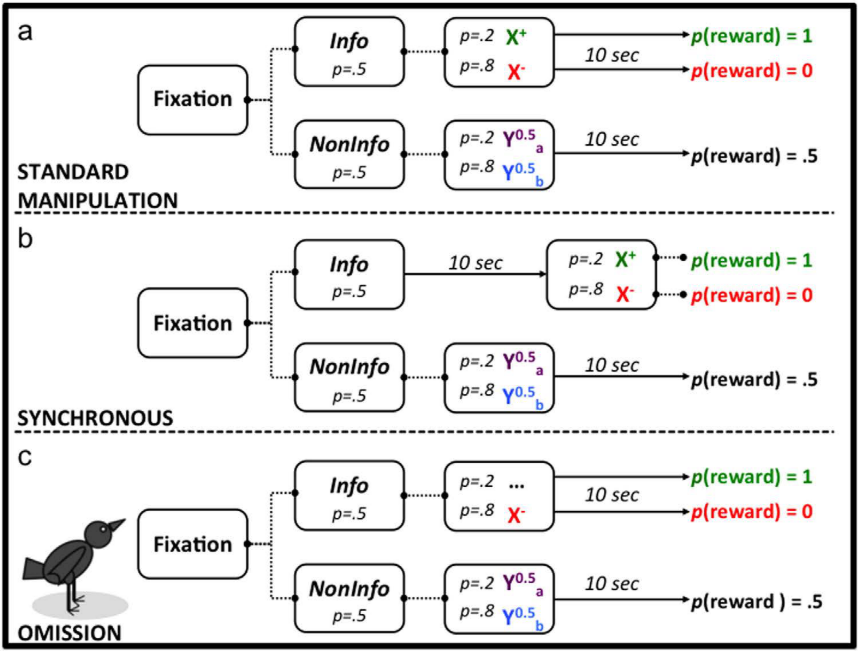
\includegraphics[scale=0.5]{Vasconcelos2015.png}
		\caption{Diseño de los experimentos 1 y 2. Las líneas punteadas indican la ausencia de demoras, y las líneas sólidas indican demora de 10s}
	\end{center}
\end{figure}


{\itshape\bfseries Experimento 1}

Había 280 ensayos forzados y 140 de elección. Los ensayos comenzaban con una luz en la tecla central. Tras una respuesta en ella se iluminaba en blanco una tecla lateral (la posición indicaba si se trataba de la alternativa informativa o la no informativa). Las probabilidades de presentación de los TL fueron .2 y .8. Tras un TF10s se apagaba la luz y se entregaba la consecuencia correspondiente.

Tras diez sesiones se corrían 4 adicionales con 20 ensayos de elección de terminal link. En estos ensayos picar la tecla central era seguido de la presentación de los siguientes pares de estímulos: $X^-\,vs\,Y^{0{.}5}_a$, $X^-\,vs\,Y^{0{.}5}_b$, $X^+\,vs\,Y^{0{.}5}_a$, y $X^+\,vs\,Y^{0{.}5}_b$; cinco de cada uno. En estos ensayos los sujetos elegían entre TLs en lugar de entre las alternativas. Una respuesta apagaba la tecla no elegida y entregaba la recompensa correspondiente.

Después, la redituabilidad de la alternativa informativa fue reducida bajando $p_{info}$, es decir la probabilidad de $X^+$, de .2 a .15, .1, .05 y 0.

{\itshape Resultados}

Este experimento pretendía probar las predicciones 1, 2 y 5. Se pretendía (a) examinar las diferencias procedimentales responsables de la elección maladaptativa, prestando atención especial al conocimiento que los starling tenían sobre las propiedades de señalización de los TL y la resistencia de su preferencia a las reducciones en probabilidad de reforzamiento; y (b) probar si las decisiones maladaptativas pueden anticiparse con los encuentro secuenciales.

{\itshape Predicción 1:} Los starlings desarrollaron rápidamente preferencia por la alternativa informativa, y la sostuvieron a pesar de disminuir la probabilidad de reforzamiento a .15 y a .1. Al disminuir a .05 se encontró mayor variabilidad, pero aun preferencia por la alternativa informativa (aunque no significativamente distinta del azar). Al llegar a 0 la preferencia se revirtió. Así, {\itshape los sujetos fueron casi insensibles a $p_{info}$, mostrando cambios solo ante valores extremos.}

{\itshape Predicción 2:} Se asume que la preferencia maladaptativa no viene de información imprecisa o incompleta sobre la probabilidades de recompensa, sino de la valoración de la información de acuerdo con su potencial para ser usada en la naturaleza. Si esto es así, las preferencias sobre los TL exclusivamente deberían reflejar un buen entendimiento de sus probabilidades de reforzamiento. Los resultados confirmaron esta predicción: $X^+ \succ Y_a^{{.}5},Y_b^{{.}5} \succ X^-$

{\itshape Predicción 5:} Las preferencias en ensayos de elección fueron cercanamente predicha por las latencias en ensayos forzados en todas las condiciones. Además, las predicciones y las preferencias parecen covariar durante la fase de adquisición.

{\itshape Discusión:} La preferencia de los starlings resistió los cambios en la probabilidad de reforzamiento. Esta preferencia no parece derivarse de un mal entendimiento de las probabilidades de reforzamiento. En todos los casos las latencias fueron buenos predictores de la elección.

{\itshape\bfseries Experimento 2}

El entrenamiento era similar salvo porque se requería una respuesta al TL para iniciar la demora de 10s en ambas alternativas en el grupo control, y en la alternativa no informativa en el grupo {\itshape sincrónico}. Una respuesta en el TL de la alternativa informativa en el grupo sincrónico terminaba el estímulo. Los grupos sincrónico y omisión diferían del grupo control en los ensayos de la alternativa informativa. En el grupo omisión se omitía el $X^+$, pero en el 20\% de los ensayos a la alternativa informativa una respuesta a la tecla lateral iluminada en blanco la apagaba y se entregaba comida tras 10s. En el 80\% restante se presentaba $X^-$ seguido de la ausencia de reforzamiento. Para el grupo sincrónico la demora de 10s ocurría entre la elección de la alternativa informativa y la entrega de información. Así, cuando se iluminaba la alternativa informativa, la primera respuesta iniciaba una demora de 10s. Una vez pasada la demora, la tecla se apagaba y se mostraba $X^+$ o $X^-$.

{\itshape Resultados}

Este experimento probó las predicciones 3, 4, y 5. La predicción 3 habla sobre la relación entre la predictabilidad de los estímulos o la duración de la incertidumbre como determinantes de la elección maladaptativa. Si el tiempo en incertidumbre es, como sugiere la explicación del forrajeo, la variable determinante, entonces arreglar la tarea de modo que el tiempo en incertidumbre sea el mismo entre las alternativas pero no se altere la correlación entre estímulos y consecuencias de la alternativa informativa debería resultar en una reversión de las preferencias, en tanto que en la ecuación 6 se elimina el tiempo bajo certidumbre de los cálculos. Al devolver ese tiempo a un estado de incertidumbre, entonces todos los tiempos de espera deberían influir la preferencia. Esto fue implementado en el grupo sincrónico.

La predicción 4 compara la lógica de la ecuación 6 con el mecanismo de contraste. Para ello se diseñó el grupo de omisión, que preserva la estructura de probabilidad del protocolo Z pero sin una señal para la recompensa segura. Bajo la lógica que lleva a la ecuación 6, la preferencia por la alternativa informativa debería prevalecer, pero bajo la hipótesis de contraste debería revertirse ({\itshape\bfseries de esto no estoy seguro; no me parece que el contraste sea dependiente de la presencia de una señal saliente como TL}).

{\itshape Predicciones 3 y 4:} El grupo con omisión en el que se elimina $X^+$ mostró inicialmente preferencia por la alternativa óptima, pero tras algunas sesiones revirtió. Parece ser que el resultado típico y paradójico aparece cuando los animales aprenden por completo las contingencias.

El grupo sincrónico, que experimentó tiempos iguales bajo incertidumbre, mostró preferencia casi exclusiva por la alternativa no informativa y óptima.

{\itshape Predicción 5:} Las predicciones del modelo de elección secuencial se ajustaron con las preferencias en los tres grupos. En el grupo de omisión, en el que hay una gran evolución temporal que incluye una reversión de preferencia, las predicciones del SCM siguieron cercanamente esos cambios.

{\itshape Discusión:} Hubo un surgimiento tardío de la preferencia en el grupo de omisión, y preferencia por la alternativa óptima en el grupo sincrónico. Parece que lo que marca la diferencia entre preferencias óptimas y subóptimas es el momento de la remoción de la incertidumbre.

{\scshape\bfseries Discusión general}

Abundan las críticas al uso de las teorías normativas, a menudo enfatizando que la optimización implica cálculos que son muy difíciles de realizar para los organismos. Estos argumentos son válidos si se dirigen a los procesos que controlan la conducta de los agentes, pero no son relevantes cuando se dirigen a los modelos de optimalidad utilizados por lo biólogos para predecir o explicar lo que los organismos realizan en la naturaleza como consecuencia de los mecanismos modelados por la selección natural. Aquí se defiende el segundo caso y se argumenta que las desviaciones de los modelos proveen material para mejorarlos.

Este análisis indica que la preferencia irracional se espera cuando los animales no incluyen los tiempos de búsqueda (ITI) y los tiempos de espera en sus cálculos. También se muestra que ignorar ambos elementos se espera cuando se toman en cuenta los mecanismos de aprendizaje. Esta aproximación es consistente con la idea de que los mecanismos de decisión son mejor entendidos cuando se toma en cuenta su interacción con la estructura de las elecciones en ambientes naturales.

{\bfseries Se defiende el uso de los cálculos de probabilidades y utilidades porque se toma en cuenta que los mecanismos son diseñados por la selección natural a través de generaciones y no se enfrentan al problema de computar soluciones óptimas en tiempo real. Los mecanismos psicológicos serían entonces equivalentes a los heurísticos propuestos por la escuela de la racionalidad limitada.}

Se mostró que si se asume que el aprendizaje depende de la expectativa de recompensa en presencia contra ausencia de un estímulo, entonces la fuerza de la asociación señal-respuesta no será afectada por los componentes comunes a todos los estímulos (como los ITI). 

En la naturaleza la información le es útil a los organismos, pero en el protocolo Z ésta no se puede usar para redirigir los esfuerzos de búsqueda. Una diferencia más entre el entorno natural y el protocolo Z es que en la naturaleza los encuentros secuenciales son la regla. 

Las cinco predicciones realizadas fueron apoyadas por los resultados experimentales. La más importante de ellas fue la desaparición de la preferencia paradójica cuando se igualó el tiempo en incertidumbre.

La conclusión es que la irracionalidad de la conducta observada en subcho proviene de evaluar a los animales en una situación en la cual la información es inútil, mientras que los procesos de decisión de los sujetos están adaptados a un mundo en el cual la información altera la conducta subsecuente. Los autores están en desacuerdo con Gigerenzer y Selten, quienes dicen que la optimalidad compite con encontrar el ``adaptive toolbox'' de organismos reales, y que nos podemos deshacer de las probabilidades y las utilidades. El agente optimizador es la selección natural, no el organismo que se comporta en tiempo real, y la optimalidad es la herramienta de los biólogos para estudiar éste enlace.

\end{document}
